\documentclass[10pt]{beamer}

\usetheme[progressbar=frametitle]{metropolis}
\usepackage{appendixnumberbeamer}

\usepackage[utf8]{inputenc}
\usepackage{booktabs}
\usepackage{array}
\usepackage{multirow}
\usepackage{chronology}

\usepackage[scale=2]{ccicons}
\usepackage{pgfplots}
\usepgfplotslibrary{dateplot}
\usepackage{xspace}
\usepackage{tikz}

\graphicspath{ {./images/} }
\newcommand{\themename}{\textbf{\textsc{metropolis}}\xspace}

\usepackage{caption}
\usepackage{amsmath}
\usepackage{amsfonts}
\usepackage{amssymb}
\usepackage{physics}
\usepackage{qcircuit}
\usepackage{relsize}
\usepackage{subfigure}

\setbeamertemplate{frametitle continuation}{\insertcontinuationcountroman}
\setbeamertemplate{bibliography item}{\insertbiblabel}

\title{Quantum Programming Languages}
\subtitle{Presentation}
% \date{\today}
\date{}
\author{Christopher Baumgartner-Trösch\\Matr.-Nr.: 11908149\\}
\institute{
        703081 SE Specialisation Seminar\\
        Supervisor: Univ.-Prof. Dr. Georg Moser\\
        SS 2024
        \\\\
        University of Innsbruck\\
        Institute of Computer Science
        \\\\
        May 24, 2024
}
% \titlegraphic{\hfill\includegraphics[height=1.5cm]{logo.pdf}}

\begin{document}

\maketitle

% \begin{frame}{Contents}
%   \setbeamertemplate{section in toc}[sections numbered]
%   \tableofcontents%[hideallsubsections]
% \end{frame}

\section{Theoretical Foundation}

\begin{frame}[fragile]{Qbit}
 \metroset{block=fill}
 % \vspace{0.25cm}
    \begin{block}{Qbit - Definition}
     A Qbit is a linear combination of the state vectors $\ket{0}$ and $\ket{1}$ multiplied with the probabilistic amplitudes $\alpha$ and $\beta$:\\
     \begin{equation*}\label{eq:alpha_beta}
	\ket{\psi} = \alpha\ket{0} + \beta \ket{1}, \quad \alpha, \beta \in \mathbb{C}^2
\end{equation*}

\begin{equation*}
    \text{where} \quad \ket{0}  = \begin{pmatrix} 1 \\ 0 \end{pmatrix} \quad \text{and} \quad \ket{1} = \begin{pmatrix} 0 \\ 1 \end{pmatrix}, \quad \ket{\psi} \in \mathbb{C}^2,
\end{equation*}

\begin{equation*}
     \text{and} \lVert \alpha \rVert^2 + \lVert \beta \rVert^2 = 1.
\end{equation*}
\end{block}
    


\begin{block}{Superposition - Definition}
    $\alpha$ and $\beta$ sufficiently describe a Qbit's state in superposition: $\begin{pmatrix} \alpha \\ \beta \end{pmatrix}$.\\
    Upon measurement, the superposition collapses to one of the state vectors.
\end{block}

\end{frame}

\begin{frame}[fragile]{System of 2 Qbits}
 \begin{equation*}
    |\Psi\rangle = \alpha|00\rangle + \beta|10\rangle + \gamma|01\rangle + \delta|11\rangle \quad \text{with} \quad |\alpha|^2 + |\beta|^2 + |\gamma|^2 + |\delta|^2 = 1
\end{equation*}

\begin{equation*}
    \ket{00}  = \begin{pmatrix} 1 \\ 0 \\ 0 \\ 0 \end{pmatrix}, \quad \ket{01} = \begin{pmatrix} 0 \\ 1 \\ 0 \\ 0 \end{pmatrix}, \quad \ket{10}  = \begin{pmatrix} 0 \\ 0 \\ 1 \\ 0 \end{pmatrix}, \quad \ket{11}  = \begin{pmatrix} 0 \\ 0 \\ 0 \\ 1 \end{pmatrix} \quad \in \quad \mathbb{C}^4
\end{equation*}
\end{frame}

\begin{frame}{Identity \& Bit Flip Gate}
\metroset{block=fill}
\begin{block}{Identity \& Bit Flip Gate}
    Read from right (input state) to left (output state $o$).\\
    Note that both $I$ and $X$ are invertible by themselves (unitary).
    \vspace{0.25cm}
    \begin{equation*}
    \Qcircuit @C=3em @R=2em {
    & & \lstick{o = b} & \gate{I} & \rstick{\ket{b}} \qw & & b \in \{0, 1\} \\
    & & \lstick{o = \neg b} & \gate{X} & \rstick{\ket{b}} \qw
    }
\end{equation*}
\end{block}

\begin{block}{Unitary}
    \begin{equation*}
    \Qcircuit @C=3em @R=2em {
    \lstick{b} & \gate{I} & \gate{I} & \rstick{\ket{b}} \qw & = & \lstick{b} & \gate{I} & \rstick{\ket{b}} \qw \\
    \lstick{b} & \gate{X} & \gate{X} & \rstick{\ket{b}} \qw & = & \lstick{b} & \gate{I} & \rstick{\ket{b}} \qw
    }
\end{equation*}
\end{block}


\end{frame}

\begin{frame}{Hadamard Gate}
\metroset{block=fill}
\begin{block}{Hadamard Gate}
    \vspace{0.25cm}
    The Hadamard gate is more interesting. It produces a \textbf{probabilistic output} with $o \stackrel{unif}{\sim} \{0, 1\}$.\\
    \vspace{0.25cm}
     \begin{equation*}
    \Qcircuit @C=3em @R=2em {
    & { \quad o = \left\{
    \begin{aligned}
    &0 \quad \text{with } \mathbb{P}(0) = \frac{1}{2} \\
    &1 \quad \text{with } \mathbb{P}(1) = \frac{1}{2}
    \end{aligned}
    \right.} &&& \lstick{o} & \gate{H} & \rstick{\ket{b}} \qw 
        & & b \in \{0, 1\}
    }
\end{equation*}
\vspace{0.5cm}
\end{block}
  
\vspace{0.25cm}

\metroset{block=fill}
\begin{block}{Quantum Phenomenon}
    \vspace{0.25cm}
    Strangly, it is also revertible by itself.
    % \vspace{0.25cm}
    \begin{equation*}
    \Qcircuit @C=3em @R=2em {
    \lstick{b} & \gate{H} & \gate{H} & \rstick{\ket{b}} \qw & = & \lstick{b} & \gate{I} & \rstick{\ket{b}} \qw
}
\end{equation*}
% \vspace{0.25cm}
\begin{equation*}
    \Qcircuit @C=3em @R=2em {
    \lstick{b} & \gate{H} & \gate{H} & \rstick{\ket{b}} \qw & = & \lstick{b} & \gate{I} & \rstick{\ket{b}} \qw
}
\end{equation*}
% \vspace{0.25cm}
\end{block}
\begin{equation*}
    \Qcircuit @C=3em @R=2em {
    & & \lstick{o = b} & \gate{Z} & \rstick{\ket{b}} \qw &
    & b \in \{0, 1\}
    }
\end{equation*}
\vspace{0.25cm}
\end{frame}

\begin{frame}{Sign Flip Gate}
    \metroset{block=fill}
    \begin{block}{Sign Flip Gate}
    \vspace{0.25cm}
\begin{equation*}
        \Qcircuit @C=3em @R=2em {
        & & \lstick{o = b} & \gate{Z} & \rstick{\ket{b}} \qw &
        & b \in \{0, 1\}
        }
\end{equation*}
\vspace{0.25cm}
\begin{equation*}
    \Qcircuit @C=3em @R=2em {
    \lstick{b} & \gate{Z} & \gate{Z} & \rstick{\ket{b}} \qw & = & \lstick{b} & \gate{I} & \rstick{\ket{b}} \qw
    }
\end{equation*}
\end{block}
\vspace{0.5cm}
\begin{block}{But: Unintuitive Behavior in Superposition}
\vspace{0.25cm}
    \begin{equation*}
    \Qcircuit @C=2em @R=2em {
    \lstick{b} & \gate{H} & \gate{Z} & \gate{H} & \rstick{\ket{b}} \qw && = && \lstick{b} & \gate{X} & \rstick{\ket{b}} \qw}
\end{equation*}
\end{block}
\end{frame}

\begin{frame}{Quantum Operations \& Bloch Sphere}

\begin{equation*}
    \ket{\psi_{\text{final}}} = \psi_{\text{final}} = \mathbf{U} \psi = \mathbf{U} \begin{pmatrix}
    U_{0,0} & U_{0,1} \\
    U_{1,0} & U_{1,1}
    \end{pmatrix} \begin{pmatrix}
    \psi_0 \\
    \psi_1
    \end{pmatrix} = \begin{pmatrix}
    U_{0,0}\psi_0 + U_{0,1}\psi_1 \\
    U_{1,0}\psi_0 + U_{1,1}\psi_1
    \end{pmatrix} \in \mathbb{C}^2.
\end{equation*}


% Ömer:
% \begin{equation*}
%     U = \sum_{i=0}^{2^n-1} \sum_{j=0}^{2^n-1} \ket{i} u_{ij} \bra{j} \quad \text{with} \quad \sum_{k=0}^{2^n-1} u_{ik}^* u_{kj} = \delta_{ij}
% \end{equation*}

\begin{figure}
    \centering
    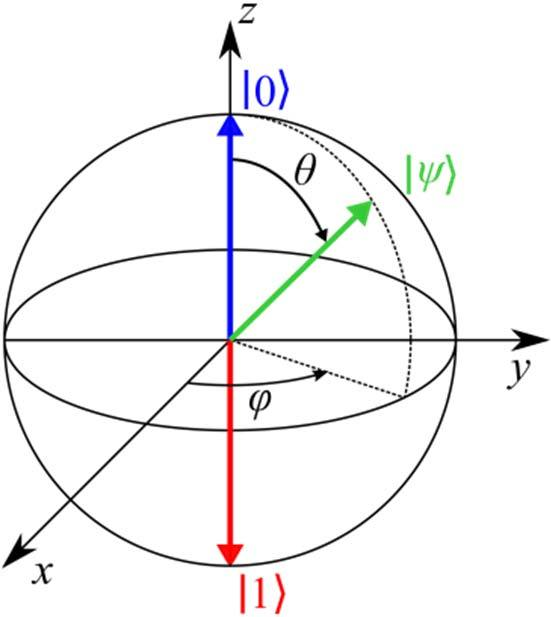
\includegraphics[width=4cm]{images/Bloch-sphere-representation-of-a-qubit.png}
    % \caption{Caption}
    \label{fig:enter-label}
\end{figure}
    
\end{frame}

\begin{frame}{Bloch Sphere}

\begin{figure}
    \hspace*{-1.1cm}
    \centering
    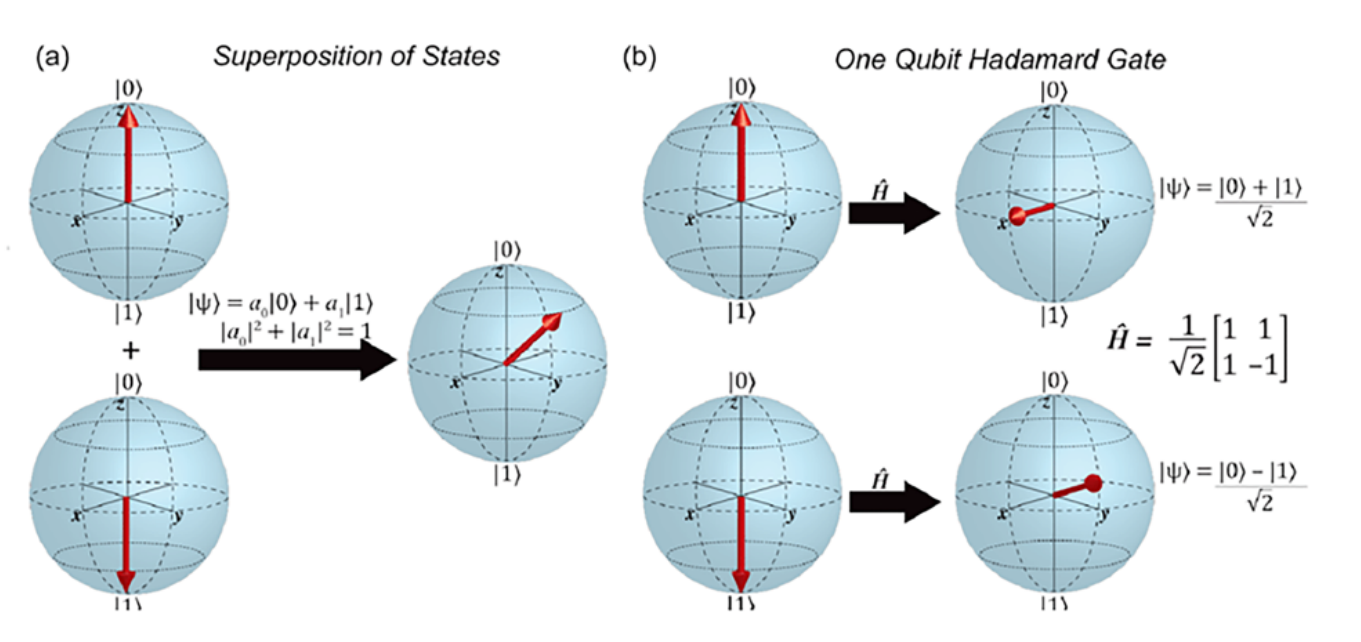
\includegraphics[width=13cm]{images/bloch-hadamard-gate.png}
    % \caption{Caption}
    \label{fig:enter-label}
\end{figure}
    
\end{frame}


% \section{Quantum Programming Languages}

% \begin{frame}{Quantum Programming Languages - Overview}
    
% \end{frame}

\section{Demo: Qiskit}


% {%
% \setbeamertemplate{frame footer}{My custom footer}
% \begin{frame}[fragile]{Frame footer}
%     \themename defines a custom beamer template to add a text to the footer. It can be set via
%     \begin{verbatim}\setbeamertemplate{frame footer}{My custom footer}\end{verbatim}
% \end{frame}
% }

% {\setbeamercolor{palette primary}{fg=black, bg=yellow}
% \begin{frame}[standout]
%   Questions?
% \end{frame}
% }

\begin{frame}[allowframebreaks]{Literature}

\nocite{kueng2023quantum}
\nocite{balamurugan_2024}
\nocite{oemer_quantum_2000}

\bibliography{bibliography}

\bibliographystyle{unsrt}
  % \nocite{umbrella, UAS, robust_intel_swarm, deep_learning_IoT, mesh_networks, swarm_intel_UAV, molloy_reed_graph}

\end{frame}

\end{document}
